
%%%%%%%%%%%%%%%%%%%%%%% file typeinst.tex %%%%%%%%%%%%%%%%%%%%%%%%%
%
% This is the LaTeX source for the instructions to authors using
% the LaTeX document class 'llncs.cls' for contributions to
% the Lecture Notes in Computer Sciences series.
% http://www.springer.com/lncs       Springer Heidelberg 2006/05/04
%
% It may be used as a template for your own input - copy it
% to a new file with a new name and use it as the basis
% for your article.
%
% NB: the document class 'llncs' has its own and detailed documentation, see
% ftp://ftp.springer.de/data/pubftp/pub/tex/latex/llncs/latex2e/llncsdoc.pdf
%
%%%%%%%%%%%%%%%%%%%%%%%%%%%%%%%%%%%%%%%%%%%%%%%%%%%%%%%%%%%%%%%%%%%


\documentclass[runningheads,a4paper,orivec]{llncs}

\usepackage{amssymb,amsmath}
\setcounter{tocdepth}{3}
\usepackage{graphicx}
\usepackage[ruled,linesnumbered]{algorithm2e}

\usepackage{url}
\urldef{\mailsa}\path|{yingqin,syshen,|
\urldef{\mailsb}\path|huadongdai,|
\urldef{\mailsc}\path|qingbowu,yanjia}@nudt.edu.cn|
\newcommand{\keywords}[1]{\par\addvspace\baselineskip
\noindent\keywordname\enspace\ignorespaces#1}

% \newtheorem{algorithm}{Algorithm}

\begin{document}

\mainmatter  % start of an individual contribution

% first the title is needed
%\title{Lecture Notes in Computer Science:\\Authors' Instructions
%for the Preparation\\of Camera-Ready
%Contributions\\to LNCS/LNAI/LNBI Proceedings}
\title{Complementary Synthesis for Encoders with Pipeline and Flow Control Mechanism}

% a short form should be given in case it is too long for the running head
%\titlerunning{Lecture Notes in Computer Science: Authors' Instructions}

% the name(s) of the author(s) follow(s) next
%
% NB: Chinese authors should write their first names(s) in front of
% their surnames. This ensures that the names appear correctly in
% the running heads and the author index.
%
\author{}
% \author{Ying Qin 
% \and ShengYu Shen \and HuaDong Dai \and QingBo Wu \and Yan Jia}

\authorrunning{}
% \authorrunning{Ying Qin %
% \and ShengYu Shen \and HuaDong Dai \and QingBo Wu \and Yan Jia}
% (feature abused for this document to repeat the title also on left hand pages)

% the affiliations are given next; don't give your e-mail address
% unless you accept that it will be published
\institute{}
% \institute{School of Computer, National University of Defense Technology, China\\
% \mailsa\mailsb\mailsc\\
% % \url{}
% }

%
% NB: a more complex sample for affiliations and the mapping to the
% corresponding authors can be found in the file "llncs.dem"
% (search for the string "\mainmatter" where a contribution starts).
% "llncs.dem" accompanies the document class "llncs.cls".
%

\toctitle{Lecture Notes in Computer Science}
\tocauthor{Authors' Instructions}
\maketitle


\begin{abstract}
Assuming that the encoder's input can be uniquely determined by its output,
complementary synthesis automatically generates its decoder
that recovers the encoder's inputs from its output.
% even if this encoder contains flow control mechanism that prevents
% its inputs from being uniquely determined by its outputs.
But the widely employed flow control mechanism
fails this assumption.
And most encoders also include pipeline stages used to improve timing.
\vspace{0.1cm}

Thus,
this paper proposes the first complementary synthesis algorithm that can generate 
pipelined decoder for encoders with flow control mechanism.
First,
it infers the flow control predicate on inputs with existing algorithm.
Second,
it finds out the pipeline stages in the encoder by enforcing the inferred flow control predicate.
% Third,
% it infers the flow control predicate for each pipeline stages.
Finally,
the decoder's Boolean functions that recover each pipeline stage and input are characterized with Craig interpolant.

\vspace{0.1cm}

Experimental results indicate that
this algorithm can always correctly generate a pipelined decoders with flow control mechanism.

\keywords{Complementary Synthesis, Flow Control Mechanism, Pipeline}
\end{abstract}


\section{Introduction}\label{sec_intro}
One of the most difficult jobs in designing communication
and multimedia chips is to design and verify complex encoder and decoder pairs.
The encoder maps its input variables $\vec{i}$ to its output variables $\vec{o}$,
% according to some predefined rules,
% such as Ethernet \cite{IEEE8023_S4} and PCI Express \cite{pcie21},
while the decoder recovers $\vec{i}$ from $\vec{o}$.
Complementary synthesis 
\cite{ShenICCAD09,ShenTCAD11,ShenTCAD12,LiuICCAD11,LiuTCAD12,TuDAC13}
eases this job by
automatically generating a decoder from an encoder,
with the assumption that $\vec{i}$ can always be
uniquely determined by a bounded sequence of $\vec{o}$.
% Thus,
% the decoder's Boolean function can be characterized
% with the algorithm proposed by Jiang et al. \cite{InterpBoolFunction}
% This algorithm constructs an unsatisfiable formula with two unrolled transition function sequences,
% both of which have the same output sequence but with different input.
% A Craig interpolant \cite{Craig} can be extracted from this unsatisfiable formula,
% and used as the decoder's Boolean function that recovers the inputs.

However,
the flow control mechanism \cite{flowcontrol} in many encoders
fails this assumption.
As shown in Figure \ref{fig_fc}a),
this mechanism prevents faster transmitter from overwhelming slower receiver
by transmitting idle symbols $I$ when the receiver can not keep up with the transmitter.
As shown in Figure \ref{fig_fc}b),
the idle symbol $I$
can only uniquely determine a small subset of inputs $\vec{i}$,
which is called flow control vector $\vec{f}$.
While the normally encoded data symbols $D_i$ can
uniquely determine all inputs, 
including both $\vec{f}$ and data vector $\vec{d}$.

Qin et al. \cite{QinTODAES15} handle such encoders by
first finding out all inputs $i\in\vec{f}$ that can by uniquely determined by $\vec{o}$,
and then inferring a flow control predicate $valid(\vec{f})$ that
% when enforced,
can make $\vec{d}$ to be uniquely determined by $\vec{o}$.

\begin{figure}[t]
\centering
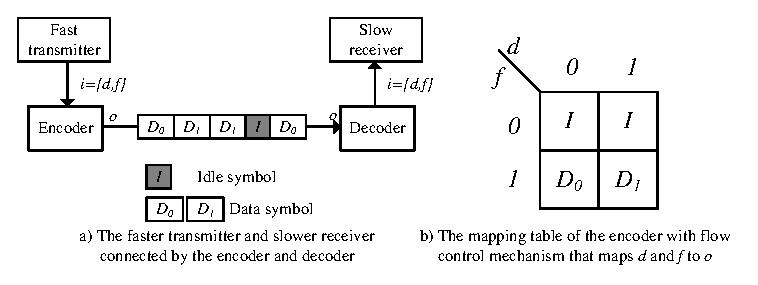
\includegraphics[width=\textwidth]{nonuniq}
\caption{Encoder with flow control mechanism}
\label{fig_fc}
\end{figure}

\begin{figure}[b]
\centering
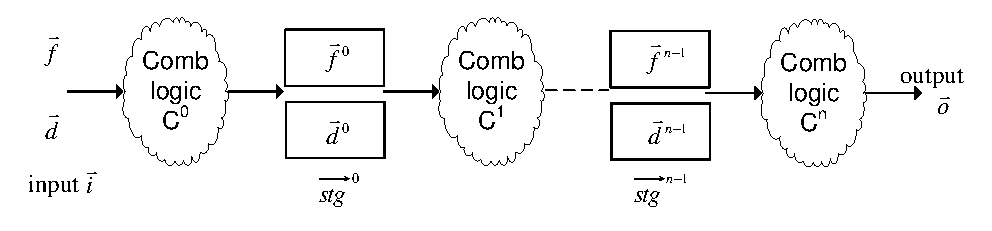
\includegraphics[width=\textwidth]{pipemod1}
\caption{Encoder with pipeline and flow control mechanism}
\label{pipemod}
\end{figure}



At the same time,
as shown in Figure \ref{pipemod},
many encoders contain
pipeline stages $\vec{stg}^j$ to cut their datapath into multiple segments $C^j$,
such that the encoder can run in higher frequency.
Just like $\vec{i}$,
each pipeline stage $\vec{stg}^j$ can also be partitioned into flow control vector $\vec{f}^j$ and data vector $\vec{d}^j$.

But the decoder generated by Qin et al. \cite{QinTODAES15} doesn't include pipeline stages,
which make it much slower than its corresponding encoder.
To overcome this problem,
this paper proposes a novel algorithm to generate pipelined decoders for flow controlled encoder.
It first applies Qin et al. \cite{QinTODAES15}'s algorithm to find out $\vec{f}$ and infers $valid(\vec{f})$.
% By assuming that each pipeline stage $\vec{stg}^j$ can be partitioned into flow control vector $\vec{f}^j$ and data vector $\vec{d}^j$,
It then finds out all $\vec{d}^j$ and $\vec{f}^j$ in each pipeline stage $\vec{stg}^j$ respectively with and without enforcing $valid(\vec{f})$.
It finally characterize the Boolean functions that recover each $\vec{stg}^j$ and $\vec{i}$ with 
Jiang et al. \cite{InterpBoolFunction}'s algorithm.

Experimental result indicates that the proposed algorithm can always 
correctly generate pipelined decoder with flow control mechanism.

\emph{The remainder of this paper is organized as follows}.
%Section \ref{sec_casestudy} explains our ideas with a simple example.
Section \ref{sec_prem} introduces the background material;
% Section \ref{sec_findfc} identifies the flow control variables,
% and infers the predicate that enables $\vec{d}$ 
% to be uniquely determined by a bounded sequence of $\vec{o}$;
Section \ref{sec_framework} introduces the overall framework of our algorithm.
Section \ref{sec_pipeinfer} finds out $\vec{f}^j$ and $\vec{d}^j$ in each pipeline stages $\vec{stg}^j$,
while Section \ref{sec_char} characterize the decoder's Boolean functions that recover each pipeline stage $\vec{stg}^j$ and the input vector $\vec{i}$.
Sections \ref{sec_exp} and \ref{sec_relwork} present the experimental results and related works;
Finally,
Section \ref{sec_conclude} sums up the conclusion.

\section{Preliminaries}\label{sec_prem}

% \subsection{Flow control mechanism}\label{subsec_fc}



\subsection{Propositional satisfiability}\label{subsec_SAT}
% We use a denotation similar to that of \cite{TuDAC13}.
The Boolean value set is denoted as $\mathbb{B}=\{0,1\}$.
A vector of variables is represented as $\vec{v}=(v,\dots)$.
The number of variables in $\vec{v}$ is denoted as $|\vec{v}|$.
If a variable $v$ is a member of $\vec{v}$,
% that is $\vec{v}=(\dots,v,\dots)$,
then we say $v\in\vec{v}$;
otherwise we say $v\notin\vec{v}$.
For a variable $v$ and a vector $\vec{v}$,
if $v\notin\vec{v}$,
then the new vector that contains both $v$ and all members of $\vec{v}$ is denoted as $v\cup\vec{v}$.
If $v\in \vec{v}$,
then the new vector that contains all members of $\vec{v}$ except $v$,
is denoted as $\vec{v}-v$.
For the two vectors $\vec{a}$ and $\vec{b}$,
the new vector with all members of $\vec{a}$ and $\vec{b}$ is denoted as $\vec{a}\cup\vec{b}$.
% The set of truth valuations of $\vec{v}$ is denoted as $[\![\vec{v}]\!]$,
% for instance,
% $[\![(v_1,v_2)]\!]=\{(0,0),(0,1),(1,0),(1,1)\}$.

% A Boolean formula $F$ over a variable set $V$ is constructed by connecting variables from $V$ 
% with symbols $\neg$, $\wedge$, $\vee$ and $\Rightarrow$,
% which stand for logical connectives negation, conjunction, disjunction, and implication, respectively.

The propositional satisfiability problem (SAT) for a Boolean formula $F$ over a variable set $V$ 
is to find a satisfying assignment $A:V\to \mathbb{B}$,
so that $F$ can be evaluated to $1$.
If $A$ exists, then $F$ is satisfiable;
otherwise,
it is unsatisfiable.

% A computer program that decides the existence of such a satisfying assignment is called a SAT solver,
%  such as Zchaff\cite{CHAFF},
%  Grasp\cite{grasp},
%  Berkmin\cite{BERKMIN},
%  and MiniSat\cite{EXTSAT}.
 
% Normally,
% a SAT solver requires the formula to be represented in the conjunctive normal form(CNF),
% in which a formula is a conjunction of its clause set,
% and a clause is a disjunction of its literal set,
% and a literal is a variable or its negation.
% A formula in the CNF format is also called a SAT instance,


% \subsection{Cofactoring}\label{subsec_pre_cofact}

% For a Boolean function $f:B^n\to B$,
% we use $supp(f)$ to denote its support set $\{v_1\dots v_n\}$.
% According to \cite{EFFSATUSMCCO},
% the positive and negative cofactors of $f(v_1\dots v\dots v_n)$ with respect to variable
% $v$ are $f_{v\equiv 1}=f(v_1\dots 1\dots v_n)$ and $f_{v\equiv 0}=f(v_1\dots 0\dots v_n)$.
% % respectively.
% % Existential quantification of $f(v_1\dots v\dots v_n)$ with respect to a
% % variable $v$ is $\exists v f=f_v+f_v’$.
% \textbf{Cofactoring} is the action that applies 1 or 0 to $v$ to get $f_{v\equiv 1}$ or $f_{v\equiv 0}$.

% \subsection{Craig interpolation}\label{subsec_pre_interp}
% Craig\cite{Craig} had proved the following theorem:
% \begin{theorem}[Craig Interpolation Theorem\cite{Craig}]\label{thm_craig}
Given two Boolean formulas $\phi_A$ and $\phi_B$,
with $\phi_A\wedge \phi_B$ unsatisfiable,
there exists a formula $\phi_I$ referring only
to the common variables of $\phi_A$ and $\phi_B$ such that $\phi_A\Rightarrow \phi_I$
and $\phi_I\wedge \phi_B$ is unsatisfiable.
We call $\phi_I$ the \textbf{interpolant} \cite{Craig} of $\phi_A$ with respect to $\phi_B$
% \end{theorem}
and use McMillan's algorithm \cite{interp_McMillan} to generate it.




\subsection{Finite state machine}\label{subsec_fsm}



The encoder is modeled by a finite state machine(FSM) $M=(\vec{s},\vec{i},\vec{o},T)$,
consisting of a state variable vector $\vec{s}$,
% an initial state $s_0\in S$,
an input variable vector $\vec{i}$,
% a finite set of configuration letters $C$,
an output variable vector $\vec{o}$,
% and a transition function $T: [\![\vec{s}]\!]\times [\![\vec{i}]\!]\to [\![\vec{s}]\!]\times [\![\vec{o}]\!]$ 
and a transition function $T: \vec{s}\times \vec{i}\to \vec{s}\times \vec{o}$ 
that computes the next state and output variable vector from the current state and input variable vector.

% As shown in Figure \ref{mealy},
% as well as in the remainder of this paper,
% the state is represented as a gray round corner box,
% and the transition function $T$ is represented as a white rectangle.
The behavior of FSM $M$ can be reasoned by unrolling transition function.
The state variable $s\in\vec{s}$, input variable $i\in\vec{i}$ and output variable $o\in\vec{o}$ at the $n$-th step 
are respectively denoted as $s_n$, $i_n$ and $o_n$.
Furthermore,
the state, the input and the output variable vectors at the $n$-th step are respectively denoted as $\vec{s}_n$, $\vec{i}_n$ and $\vec{o}_n$.
% We further denote the sequence of state, input letter and output letter from the $n$-th to the $m$-th step respectively as $s_n^m$, $i_n^m$ and $o_n^m$.
A \textbf{path} is a state sequence $<\vec{s}_n,\dots,\vec{s}_m>$ with $\exists \vec{i}_j\vec{o}_j (\vec{s}_{j+1},\vec{o}_j)\equiv T(\vec{s}_j,\vec{i}_j)$ for all $n\le j< m$.
A \textbf{loop} is a path $<\vec{s}_n,\dots,\vec{s}_m>$ with $\vec{s}_n\equiv \vec{s}_m$.



\subsection{The algorithm to find out flow control vector $\vec{f}$}\label{subsec_chkextdec}


Qin et al. \cite{QinTODAES15} proposed a halting algorithm
to find out $\vec{f}$ by iteratively calling 
an under-approximative and an over-approximative approaches.
% The first one is an under-approximative one that presented in \ref{subsub_sound},
% while the second one is an over-approximative one presented in \ref{subsub_complete}.
% We will present these two approaches below and show 
% that they will eventually converge.

\subsubsection{The under-approximative approach}\label{subsub_sound}
As shown in Figure \ref{fig_pc}a),
on the unrolled transition functions,
an input variable $i\in\vec{i}$ can be uniquely determined,
if there exist three integers $p$, $l$ and $r$,
such that for any particular valuation of the output sequence $<\vec{o}_p,\dots,\vec{o}_{p+l+r}>$,
$i_{p+l}$ cannot be 0 and 1 at the same time.
This is equal to the unsatisfiability of $F_{PC}(p,l,r)$ in Equation (\ref{uniqt1}).

\begin{equation}\label{uniqt1}
% \begin{split}
F_{PC}(p,l,r):=
\left\{
\begin{array}{cc}
&\bigwedge_{m=0}^{p+l+r}
\{
(\vec{s}_{m+1},\vec{o}_m)\equiv T(\vec{s}_m,\vec{i}_m)
\}
\\
\wedge&\bigwedge_{m=0}^{p+l+r}
\{
(\vec{s'}_{m+1},\vec{o'}_m)\equiv T(\vec{s'}_m,\vec{i'}_m)
\}
\\
\wedge&\bigwedge_{m=p}^{p+l+r}\vec{o}_m\equiv \vec{o'}_m \\
\wedge& i_{p+l}\equiv 1 \wedge  i'_{p+l}\equiv 0 
% \wedge&\bigwedge_{m=0}^{p+l+r}assertion(\vec{i}_m) \\
% \wedge&\bigwedge_{m=0}^{p+l+r}assertion(\vec{i'}_m) 
\end{array}
\right\}
% \end{split}
\end{equation}

\begin{figure}[t]
\begin{center}
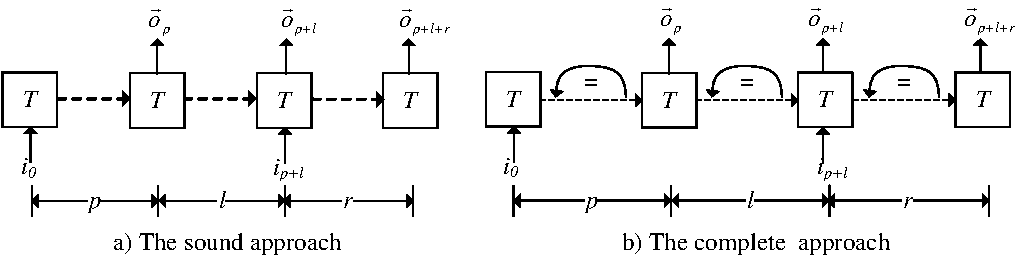
\includegraphics[width=\textwidth]{pc}
\end{center}
\caption{The under and over-approximative approaches}
  \label{fig_pc}
\end{figure}


% Here,
% $p$ is the length of the prefix state transition sequence.
% $l$ and $r$ are the lengths of the two output sequences 
% $<\vec{o}_{p+1},\dots,\vec{o}_{p+l}>$ and $<\vec{o}_{p+l+1},\dots,\vec{o}_{p+l+r}>$
% used to determine $i_{p+l}$.
Line 1 of Equation (\ref{uniqt1}) corresponds to the path in Figure \ref{fig_pc}a),
while Line 2 is a copy of it.
% These two paths are of the same length.
Line 3 forces these two paths' output sequences to be the same,
while Line 4 forces their $i_{p+l}$ to be different.
% Line 5 and 6 are the assertion predicates given 
% by the user that constrain the valid valuation on $\vec{i}$.
% PC in $F_{PC}$ is the abbreviation of "parameterized complementary",
% which means $F_{PC}(p,l,r)$ is used to check whether the encoder's input can be uniquely determined with the three parameters $p$, $l$ and $r$.


% According to Figure \ref{fig_pc}a),
% the first three lines of Equation (\ref{uniqt1}) are two unrolled transition function sequences with the same output sequences.
% They can always be satisfied with the same input variable vectors and initial state vector.
% And the last two lines are constraints on input variable vectors.
% We always check their satisfiability before running our algorithm.
% So the unsatisfiability of $F_{PC}(p,l,r)$ always means $i_{p+l}\equiv i'_{p+l}$.
% 
% 
% % According to Figure \ref{fig_pc},
% % % it is obvious that,
% % if $F_{PC}(p,l,r)$ is unsatisfiable,
% % then $F_{PC}(p',l',r')$ is also unsatisfiable for $p'\ge p$, $l'\ge l$ and $r'\ge r$.
% According to Equation (\ref{uniqt1}),
% % and Figure \ref{fig_pc},
% % we can find that,
% for $p'\ge p$, $l'\ge l$ and $r'\ge r$,
% the clause set of $F_{PC}(p',l',r')$ is a super set of $F_{PC}(p,l,r)$.
% % This also lead to the same conclusion.
% % This means,
% So,
% the bounded proof of $F_{PC}(p,l,r)$'s unsatisfiability
% can be generalized to unbounded cases.
% 
% \begin{proposition}\label{prop_pc1}
% If $F_{PC}(p,l,r)$ is unsatisfiable,
% % then $i_{p+l}$ cannot take on two different values for any particular valuation of the output sequence $<\vec{o}_{p},\dots,\vec{o}_{p+l+r}>$,
% then $i_{p+l}$ can be uniquely determined by $<\vec{o}_{p},\dots,\vec{o}_{p+l+r}>$ for all larger $p$, $l$ and $r$.
% \end{proposition}



\subsubsection{The over-approximative approach}\label{subsub_complete}
For $F_{PC}(p,l,r)$ presented above,
there are two possibilities:
\textbf{(1)}. $i_{p+l}$ can be uniquely determined by $<\vec{o}_{p},\dots,\vec{o}_{p+l+r}>$ for some $p$, $l$ and $r$;
or \textbf{(2)}. $i_{p+l}$ can't be uniquely determined for any $p$, $l$ and $r$.

% \begin{enumerate}
%  \item 
% $i_{p+l}$ can be uniquely determined by $<\vec{o}_{p},\dots,\vec{o}_{p+l+r}>$ for some $p$, $l$ and $r$;
%  \item 
% $i_{p+l}$ can't be uniquely determined by $<\vec{o}_{p},\dots,\vec{o}_{p+l+r}>$ for any $p$, $l$ and $r$.
% \end{enumerate}

For the 1st case,
by iteratively increasing  $p$, $l$ and $r$,
$F_{PC}(p,l,r)$ will eventually become unsatisfiable.
But for the 2nd case,
this method will never terminate.
So,
to obtain a halting algorithm,
we need the approach shown in Figure \ref{fig_pc}b) to check the 2nd case,
which is similar to Figure \ref{fig_pc}a) but with three additional constraints used to detect loops 
on the three state sequences $<\vec{s}_{0},\dots,\vec{s}_{p}>$, $<\vec{s}_{p+1},\dots,\vec{s}_{p+l}>$ and 
$<\vec{s}_{p+l+1},\dots,\vec{s}_{p+l+r}>$.
It is formally defined in Equation (\ref{uniqln}) 
with the last three lines corresponding to the three new constraints.
If it is satisfiable,
then by unrolling these three loops,
we can prove the 2nd case.

\begin{equation}\label{uniqln}
% \begin{split}
F_{LN}(p,l,r):=\\
\left\{
\begin{array}{cc}
&F_{PC}(p,l,r)\\
\wedge&\bigvee_{x=0}^{p-1}\bigvee_{y=x+1}^{p} \{\vec{s}_x\equiv \vec{s}_y\wedge \vec{s'}_x\equiv \vec{s'}_y\} \\
\wedge&\bigvee_{x=p+1}^{p+l-1}\bigvee_{y=x+1}^{p+l} \{\vec{s}_x\equiv \vec{s}_y\wedge \vec{s'}_x\equiv \vec{s'}_y\} \\
\wedge&\bigvee_{x=p+l+1}^{p+l+r-1}\bigvee_{y=x+1}^{p+l+r} \{\vec{s}_x\equiv \vec{s}_y\wedge \vec{s'}_x\equiv \vec{s'}_y\}
\end{array}
\right\}
% \end{split}
\end{equation}

% LN in $F_{LN}$ stands for "loop non-complementary",
% which means $F_{LN}(p,l,r)$ with three loops is used to check whether 
% the input variable can NOT be uniquely determined.


% When $F_{LN}(p,l,r)$ is satisfiable,
% then $i_{p+l}$ can't be uniquely determined by $<\vec{o}_{p},\dots,\vec{o}_{p+l+r}>$.
% More importantly,
% by unrolling these three loops,
% we can generalize the satisfiability of $F_{LN}(p,l,r)$ to all larger $p$, $l$ and $r$.
% This means:
% 
% 
% \begin{proposition}\label{prop_ln1}
% If $F_{LN}(p,l,r)$ is satisfiable,
% then $i_{p+l}$ cannot be uniquely determined by $<\vec{o}_{p},\dots,\vec{o}_{p+l+r}>$ for all larger $p$, $l$ and $r$.
% \end{proposition}

\subsubsection{Identifying flow control vector $\vec{f}$ with Algorithm \ref{alg_fofc}}\label{subsubsec_findfc}
% To facilitate the presentation of our algorithm,
% We assume that the input variable vector $\vec{i}$ can be partitioned into 
% the flow control vector $\vec{f}$ and the data vector $\vec{d}$.
% The flow control vector $\vec{f}$ is used to indicate the validness of $\vec{d}$.
% So,
% for a properly designed encoder,
% $\vec{f}$ should always be uniquely determined by a bounded sequence of the encoder's output vector $\vec{o}$,
% or else the decoder cannot recognize the validness of $\vec{d}$.
% 
% Thus,
% Algorithm \ref{alg_fofc} is proposed to identify $\vec{f}$.
% At Line \ref{initfd},
% the initial value of $f$ and $d$ are set to empty vector.
% At Line \ref{initplr},
% the initial value of $p$, $l$ and $r$ are all set to 0.
% At Line \ref{while},
% a while loop is used to iterate on all $i\in\vec{i}$.
At Line \ref{adduniq},
the input $i$ that can be uniquely determined will be moved to vector $\vec{f}$.
% On the other hand,
If $F_{LN}(p,l,r)$ is satisfiable at Line \ref{nonuniqres},
the input $i$ that can NOT be uniquely determined will be moved to vector $\vec{d}$.
Please refer to \cite{QinTODAES15} for its termination and correctness proof.

\begin{algorithm}[t]
\SetAlgoVlined
\KwIn{The input variable vector $\vec{i}$.}
\KwOut{$\vec{f}\subset \vec{i}$, and the maximal $p$, $l$ and $r$ reached in this searching.}
$\vec{f}: = \{\}$;$\vec{d}:= \{\}$;$p$:= 0 ;~$l$:= 0 ;~$r$:= 0 \;
\ShowLnLabel{while}\While{$\vec{i}\ne \{\}$}{
  assume $i\in\vec{i}$\;
  $p++$; ~ $l++$; ~ $r++$\;
  \uIf {$F_{PC}(p,l,r)$ is unsatisfiable for $i$} {
    \ShowLnLabel{adduniq}
    $\vec{f}:= i\cup\vec{f}$ ; ~
    $\vec{i}:=\vec{i}-i$\;
  }\ShowLnLabel{nonuniqres}
  \ElseIf {$F_{LN}(p,l,r)$ is satisfiable for  $i$}{
    $\vec{d}:=i\cup\vec{d}$ ; ~
    $\vec{i}:=\vec{i}-i$
  }
}
\KwRet ($\vec{f}$, $p$, $l$, $r$)
\caption{Identifying the flow control vector $\vec{f}$}
\label{alg_fofc}
\end{algorithm}


% \section{Inferring the flow control predicate $valid(\vec{f})$}


% Furthermore,
% the validness of $\vec{d}$ is indicated by a predicate $valid(\vec{f})$.
% So for a properly designed encoder,
% $valid(\vec{f})$ should make $\vec{d}$ to be uniquely determined by the encoder's output.

% In Subsection \ref{subsec_craig},
% we propose  an algorithm 
% to characterize a Boolean function that makes a Boolean formula satisfiable.
% In Subsection \ref{subsec_infer},
% we apply this algorithm to infer $valid(\vec{f})$,
% % the predicate that enable $\vec{d}$ to be uniquely determined by a bounded sequence of $\vec{o}$.
% the predicate that enables $\vec{d}$ to be uniquely determined.


\subsection{Inferring $valid(\vec{f})$ that enables $\vec{d}$ to be uniquely determined}\label{subsec_infer}
% This subsection introduces the non-trivial details of how to infer the predicate $valid(\vec{f})$.
% So we first present an intuitive and informal introduction in \ref{subsub_intro}.
% And then present its details in \ref{subsub_nonloop}, \ref{subsub_loop} and \ref{subsub_overal}.

% \subsubsection{\textbf{Intuitive introduction}}\label{subsub_intro}.

% In this section,
% we will present how to compute the predicate $valid(\vec{f})$ that enables $\vec{d}$ to be uniquely determined.

This is also proposed by Qin et al. \cite{QinTODAES15}.
It first introduces Algorithm \ref{alg_craigchar} to characterize a function 
that makes a Boolean formula satisfiable.
And then as shown in Figure \ref{fig_mono},
Algorithm \ref{alg_craigchar} is used to characterize $\neg FSAT_{PC}(p,l,r)$,
a monotonically growing under-approximation of $valid(\vec{f})$,
and $\neg FSAT_{LN}(p,l,r)$,
a monotonically shrinking over-approximation of $valid(\vec{f})$.
And finally we show that these two approximations will eventually converge to $valid(\vec{f})$.
% Please refer to \cite{QinTODAES15} for the proof of its correctness and termination.



\subsubsection{Characterizing a function that makes a Boolean formula satisfiable}\label{subsubsec_craig}

For a particular Boolean relation $R(\vec{a},\vec{b},t)$, 
with $R(\vec{a},\vec{b},0)\wedge R(\vec{a},\vec{b},1)$ unsatisfiable.
Algorithm \ref{alg_craigchar} characterize a Boolean function $FSAT_R(\vec{a})$
that covers and only covers all the valuations of $\vec{a}$ 
that can make $R(\vec{a},\vec{b},1)$ satisfiable.
Line \ref{testsat} finds out new valuation of $\vec{a}$ that can make $R(\vec{a},\vec{b},1)$ satisfiable,
but hasn't been covered by $FSAT_R(\vec{a})$.
Lines \ref{cofact1}, \ref{cofact2} and \ref{ab} enlarge this valuation 
to an interpolant $ITP(\vec{a})$ with McMillan's algorithm \cite{interp_McMillan}.
Line \ref{add} adds $ITP(\vec{a})$ to $FSAT_R(\vec{a})$.
% It is formally defined below:

% we have the following two assumptions:
% \begin{enumerate}
% \item \textbf{Assumption 1} :
% $R(\vec{a},\vec{b},0)\wedge R(\vec{a},\vec{b},1)$ is unsatisfiable.
% % That is,
% % $\vec{a}$ and $\vec{b}$ uniquely determine $t$.
% $\vec{a}$ and $\vec{b}$ are respectively called the important and the non-important variable vectors,
% $t$ is the target variable.
% \item \textbf{Assumption 2} :
% $R(\vec{a},\vec{b},t)$ is satisfiable for all valuations of $\vec{a}$.
% \end{enumerate}
% 
% In the remainder of this paper, 
% when we use the algorithm introduced in this subsection,
% we will show that these two assumptions are fulfilled.


% \begin{equation}\label{fchar}
% % \begin{split}
% FSAT_R(\vec{a}):=
% \left\{
% \begin{array}{rcl}
% 1 & & \exists\vec{b}.R(\vec{a},\vec{b},1) \\
% 0 & & otherwise
% \end{array}
% \right.
% % \end{split}
% \end{equation}
%% HAHA come to here

% Thus,
% a naive algorithm of computing $FSAT_R(\vec{a})$ is to enumerate all valuations of $\vec{a}$,
% and collect all those valuations that make $R(\vec{a},\vec{b},1)$ satisfiable.
% But the number of valuations to be enumerated is $2^{|\vec{a}|}$,
% which will prevent this algorithm from terminating within reasonable time for a large $\vec{a}$.

% We can speed up this naive algorithm by expanding each valuation of $\vec{a}$ 
% to a larger set with cofactoring \cite{EFFSATUSMCCO} and Craig interpolant \cite{interp_McMillan}.
% Intuitively,
% assume that $R(\vec{a},\vec{b},1)$ is satisfiable with a satisfying assignment $A:\vec{a}\cup\vec{b}\cup\{t\}\to\{0,1\}$,
% the following new formula can be constructed by cofactoring \cite{EFFSATUSMCCO}:



% \begin{equation}
% % \begin{split}
% R(\vec{a},A(\vec{b}),1):=R(\vec{a},\vec{b},1)_{b\equiv A(b)}
% % \end{split}
% \end{equation}

% Assume $A:\vec{a}\cup\vec{b}\cup\{t\}\to \mathbb{B}$ is a satisfying assignment of $R(\vec{a},\vec{b},1)$.
% % Because $R(\vec{a},A(\vec{b}),0)\wedge R(\vec{a},A(\vec{b}),1)$ is unsatisfiable,
% According to Subsection \ref{subsec_SAT},
% the interpolant $ITP(\vec{a})$ of $R(\vec{a},A(\vec{b}),1)$ with respect to $R(\vec{a},A(\vec{b}),0)$ 
% % used as an over-approximation of the set of $\vec{a}$ that makes $R(\vec{a},A(\vec{b}),1)$ satisfiable.
% % At the same time,
% % $ITP(\vec{a})\wedge R(\vec{a},A(\vec{b}),0)$ is unsatisfiable,
% % so $ITP(\vec{a})$ covers nothing that can make $R(\vec{a},A(\vec{b}),0)$ satisfiable.
% % Thus,
% covers all $\vec{a}$ that can make $R(\vec{a},A(\vec{b}),1)$ satisfiable.


% Based on the foregoing discussion,

% 
% Each iteration of the while loop in Algorithm \ref{alg_craigchar} adds at least a valuation of $\vec{a}$ to $FSAT_R(\vec{a})$,
% which means that $FSAT_R(\vec{a})$ is a Boolean function that covers a bounded and strictly increasing set of valuations of $\vec{a}$.
% So Algorithm \ref{alg_craigchar} is a halting one.


% 
% With Algorithm \ref{alg_craigchar} we can find out $FSAT_{F_{PC}}(\vec{f}_{p+l})$, 
% the set of 
% valuation of $\vec{f}_{p+l}$ that can make $F_{PC}(p,l,r)$ satisfiable for a particular $p$, $l$ and $r$.
% So its negation $\neg FSAT_{F_{PC}}(\vec{f}_{p+l})$ seems to be what we want.
% 
% As shown intuitively in Figure \ref{fig_mono},
% $\neg FSAT_{F_{PC}}(\vec{f}_{p+l})$ is an under-approximation of $valid(\vec{f})$
% that grow monotonically with respect to $p$, $l$ and $r$.
% We will prove this in \ref{subsub_nonloop}.
% So we still need an over-approximation of $valid(\vec{f})$ 
% that shrinks monotonically with respect to $p$, $l$ and $r$ to construct a halting algorithm,
% which will be presented in \ref{subsub_loop}.



% % We call the predicate that cover and only cover this set $FSAT_{PC}(p,l,r)$.
% % And we will present how to infer it in \ref{subsub_nonloop}.
% 
% % But as shown in Subsection \ref{subsec_chkextdec},
% % from the fact that $\vec{d}$ is uniquely determined for some particular $p$, $l$ and $r$,
% % we can only know that it is also uniquely determined for all larger $p'$,$l'$ and $r'$.
% % On the other hand,
% But according to Figure \ref{fig_pc} and Proposition \ref{prop_pc1},
% only the unsatisfiability of $F_{PC}(p,l,r)$ can be generalized to larger $p$, $l$ and $r$,
% while its satisfiability can't.
% % $\vec{d}_{p+l}$ not uniquely determined for some particular $p$, $l$ and $r$,
% % may become uniquely determined for larger $p$, $l$ and $r$.
% % For example,
% % an encoder with 3 step latency can't uniquely determine its input $\vec{i}$ with $p$, $l$ and $r$ smaller than 3.
% % But it can with $p$, $l$ and $r$ larger than 3.
% % That means,
% This means,
% a particular valuation of $\vec{f}_{p+l}$ that 
% makes $F_{PC}(p,l,r)$ satisfiable for some $p$, $l$ and $r$,
% may make it unsatisfiable for some larger $p$, $l$ and $r$.
% 
% So as shown in Figure \ref{fig_mono}, 
% $FSAT_{F_{PC}}(\vec{f}_{p+l})$ is a set monotonically shrinking with respect to $p$, $l$ and $r$,
% which make its negation $\neg FSAT_{PC}(p,l,r)$ an under-approximation of $valid(\vec{f})$
% that grow monotonically with respect to $p$, $l$ and $r$.
% We still need an over-approximation that shrink monotonically to construct a halting algorithm.


% Inspired by the Figure \ref{fig_ln} and $F_{LN}(p,l,r)$,
% we can compute this over-approximation by using Algorithm \ref{alg_craigchar} 
% to find out the set of valuation of $\vec{f}_{p+l}$ that can make $F_{LN}(p,l,r)$ satisfiable.
% We call the predicate that covers and only covers this set $FSAT_{LN}(p,l,r)$.
% With a satisfiable $F_{LN}(p,l,r)$,
% by unrolling the three loops in Figure \ref{fig_ln},
% we can prove that $F_{LN}(p,l,r)$ is still satisfiable for larger $p$, $l$ and $r$.
% That means $FSAT_{LN}(p,l,r)$ is a set of valuation of $\vec{f}_{p+l}$ that makes $F_{LN}(p,l,r)$ satisfiable 
% and grows monotonically with respect to $p$, $l$ and $r$.
% So as shown in Figure \ref{fig_mono},
% $\neg FSAT_{LN}(p,l,r)$ is an over-approximation of $valid(\vec{f})$ that shrinks monotonically.
% We will present how to infer it in \ref{subsub_loop}.
% 
% Together with these two inferred predicates,
% an iterative algorithm is presented in \ref{subsub_overal} to infer $valid(\vec{f})$.

\begin{algorithm}[t]
\SetAlgoVlined
\KwIn{The Boolean formula $R(\vec{a},\vec{b},t)$.
% its important variable vector $\vec{a}$,
% its non-important variable vector $\vec{b}$,
% and its target variable $t$
}
\KwOut{$FSAT_R(\vec{a})$ that makes $R(\vec{a},\vec{b},1)$ satisfiable.}
\ShowLnLabel{initcondition}
$FSAT_R(\vec{a}):= 0$ \;
\ShowLnLabel{testsat}
\While { $R(\vec{a},\vec{b},1)\wedge\neg FSAT_R(\vec{a})$ is satisfiable } {
  assume $A:\vec{a}\cup\vec{b}\cup\{t\}\rightarrow \{0,1\}$ is the satisfying assignment \;
\ShowLnLabel{cofact1}
  $\phi_A(\vec{a}):= R(\vec{a},A(\vec{b}),1)$ \;
\ShowLnLabel{cofact2}
  $\phi_B(\vec{a}):= R(\vec{a},A(\vec{b}),0)$ \;
\ShowLnLabel{ab}
  assume $ITP(\vec{a})$ is the Craig interpolant of $\phi_A$ with respect to $\phi_B$ \;
\ShowLnLabel{add}
  $FSAT_R(\vec{a}):= ITP(\vec{a}) \vee FSAT_R(\vec{a})$ \;
}
\KwRet $FSAT_R(\vec{a})$
\caption{$CharacterizingFormulaSAT(R,\vec{a},\vec{b},t)$
% :Characterizing a Boolean function over $\vec{a}$ that can make $R(\vec{a},\vec{b},1)$ satisfiable
}
\label{alg_craigchar}
\end{algorithm}

\subsubsection{Computing monotonically growing under-approximation of $valid(\vec{f})$}\label{subsub_nonloop}
By replacing $i$ in Equation (\ref{uniqt1}) with $\vec{d}$ inferred in Algorithm \ref{alg_fofc},
we have:

\begin{equation}\label{uniqt1d}
% \begin{split}
F^d_{PC}(p,l,r):=
\left\{
\begin{array}{cc}
&\bigwedge_{m=0}^{p+l+r}
\{
(\vec{s}_{m+1},\vec{o}_m)\equiv T(\vec{s}_m,\vec{i}_m)
\}
\\
\wedge&\bigwedge_{m=0}^{p+l+r}
\{
(\vec{s'}_{m+1},\vec{o'}_m)\equiv T(\vec{s'}_m,\vec{i'}_m)
\}
\\
\wedge&\bigwedge_{m=p}^{p+l+r}\vec{o}_m\equiv \vec{o'}_m \\
\wedge& \vec{d}_{p+l}\ne \vec{d}'_{p+l} \\
% \wedge&\bigwedge_{m=0}^{p+l+r}assertion(\vec{i}_m) \\
% \wedge&\bigwedge_{m=0}^{p+l+r}assertion(\vec{i'}_m) 
\end{array}
\right\}
% \end{split}
\end{equation}

% Here,
% $\vec{d}_{p+l}\ne \vec{d}'_{p+l}$ means some bit in $\vec{d}_{p+l}$ 
% isn't equal to the corresponding bit in $\vec{d}'_{p+l}$.
If $F^d_{PC}(p,l,r)$ is satisfiable,
then $\vec{d}_{p+l}$ can't be uniquely determined by $<\vec{o}_p,\dots,\vec{o}_{p+l+r}>$.
We define $T_{PC}(p,l,r)$ by collecting the 3rd line of (\ref{uniqt1d}):

\begin{equation}\label{tpc}
% \begin{split}
T_{PC}(p,l,r):=\\
\left\{
\begin{array}{cc}
      &\bigwedge_{m=p}^{p+l+r}\vec{o}_m\equiv \vec{o'}_m \\
\end{array}
\right\}
% \end{split}
\end{equation}

\begin{figure}[b]
\begin{center}

\includegraphics[width=0.5\textwidth]{mono}
\end{center}
\caption{The monotonicity of $FSAT_{PC}(p,l,r)$ and $FSAT_{LN}(p,l,r)$}
  \label{fig_mono}
\end{figure}

By substituting $T_{PC}(p,l,r)$ back into $F^d_{PC}(p,l,r)$,
we have a new formula:
\begin{equation}\label{fpcq}
% \begin{split}
F'^d_{PC}(p,l,r,t):=
\left\{
\begin{array}{cc}
&\bigwedge_{m=0}^{p+l+r}
\{
(\vec{s}_{m+1},\vec{o}_m)\equiv T(\vec{s}_m,\vec{i}_m)
\}
\\
\wedge&\bigwedge_{m=0}^{p+l+r}
\{
(\vec{s'}_{m+1},\vec{o'}_m)\equiv T(\vec{s'}_m,\vec{i'}_m)
\}
\\
\wedge& t\equiv T_{PC}(p,l,r)\\
\wedge& \vec{d}_{p+l}\ne \vec{d'}_{p+l} \\
% \wedge&\bigwedge_{m=0}^{p+l+r}assertion(\vec{i}_m) \\
% \wedge&\bigwedge_{m=0}^{p+l+r}assertion(\vec{i'}_m) 
\end{array}
\right\}
% \end{split}
\end{equation}


Obviously $F^d_{PC}(p,l,r)$ and $F'^d_{PC}(p,l,r,1)$ are equivalent.
% $\vec{d}$ cannot be uniquely determined for a particular valuation of $p$, $l$ and $r$ if $F'_{PC}(p,l,r,1)$ is satisfiable.
We further define:

% By comparing Equation (\ref{fpcq}),
% it is obvious that $F_{PC}(p,l,r)$ in Equation (\ref{uniqt1}) can be reformulated as: 
% \begin{equation}\label{fpcref}
% % \begin{split}
% F_{PC}(p,l,r):=F'_{PC}(p,l,r,t)\wedge (t\equiv 1)
% \end{equation}
% 
% $\vec{f}_{p+l}$ can be uniquely determined by $<\vec{o}_p,\dots,\vec{o}_{p+l+r}>$,
% so $\vec{f}_{p+l}\equiv \vec{f'}_{p+l}$ always holds.
% Thus,
% $\vec{i}_{p+l}\ne \vec{i'}_{p+l}$ in Line 3 of Equation (\ref{fpcq}) should be reformulated as $\vec{d}_{p+l}\ne \vec{d'}_{p+l}$.


% Thus,
% to use Algorithm \ref{alg_craigchar} to characterize the formula over $\vec{f}_{p+l}$ that makes $F'_{PC}(p,l,r,1)$ satisfiable,
% we can define the following equation:
\begin{equation}\label{pcdef1}
\vec{a}:=\vec{f}_{p+l}
\end{equation}

\begin{equation}\label{pcdef2}
\vec{b}:=\vec{d}_{p+l}\cup \vec{d'}_{p+l}\cup \vec{s}_0\cup \vec{s'}_0\cup\bigcup_{0\le x\le p+l+r,x\neq (p+l)}(\vec{i}_{x}\cup\vec{i'}_{x})
\end{equation}

% $\vec{f}_{p+l}$ can be uniquely determined, 
% so we don't need to consider $\vec{f'}_{p+l}$.
Thus,
$\vec{a}\cup\vec{b}$ is the vector that contains all the input variable vectors $<\vec{i}_0,\dots,\vec{i}_{p+l+r}>$ and $<\vec{i'}_0,\dots,\vec{i'}_{p+l+r}>$
at all steps for the two sequences of unrolled transition function.
It also contains the two initial states $\vec{s}_0$ and $\vec{s'}_0$.
% In addition,
% the transition function $T$ in the first two lines of Equation (\ref{fpcq})
% is a function that computes the next state and the output variable vector from the current state and input variable vector.
So $\vec{a}$ and $\vec{b}$ can uniquely determine the value of $t$ in $F'^d_{PC}(p,l,r,t)$,
% That is,
% With $\vec{a}$ defined in (\ref{pcdef1}),
% $\vec{b}$ defined in (\ref{pcdef2})
% and $F'^d_{PC}(p,l,r,t)$ as $R(\vec{a},\vec{b},t)$,
which means $R(\vec{a},\vec{b},1)\wedge R(\vec{a},\vec{b},0)$ is unsatisfiable.
Thus,
for a particular combination of $p$, $l$ and $r$,
the Boolean function over $\vec{f}_{p+l}$ that makes $F'^d_{PC}(p,l,r,1)$ satisfiable can be computed 
by calling Algorithm \ref{alg_craigchar} with $F'^d_{PC}(p,l,r,t)$, $\vec{a}$ and $\vec{b}$ defined above:

\begin{equation}\label{fsat_pc}
FSAT_{PC}(p,l,r):=CharacterizingFormulaSAT(F'^d_{PC}(p,l,r,t),\vec{a},\vec{b},t)
\end{equation}

% So $FSAT_{PC}(p,l,r)$ is the set of $\vec{f}_{p+l}$ 
% that makes $F^d_{PC}(p,l,r)$ satisfiable.
% Thus,
% its negation $\neg FSAT_{PC}(p,l,r)$ is the set of $\vec{f}_{p+l}$ 
% that makes $F^d_{PC}(p,l,r)$ unsatisfiable.
% 
% Again according to Proposition \ref{prop_pc1},
% the unsatisfiable proof of $F^d_{PC}(p,l,r)$ can be generalized to all larger $p$, $l$ and $r$.
% So every valuation of $\vec{f}$ covered by $\neg FSAT_{PC}(p,l,r)$ can also make $F^d_{PC}(p,l,r)$ unsatisfiable for all larger $p$, $l$ and $r$.
As shown in Figure \ref{fig_mono},
% we have:
% \begin{proposition}\label{prop_pc}
$\neg FSAT_{PC}(p,l,r)$ is an under-approximation of $valid(\vec{f})$ monotonically growing with respect to 
$p$, $l$ and $r$.
% \end{proposition}




\subsubsection{Computing monotonically shrinking over-approximation of $valid(\vec{f})$}\label{subsub_loop}
Similarly,
we can define :
% by replacing $i$ in $F_{LN}(p,l,r)$ of Equation (\ref{uniqln}) with $\vec{d}$,
% we have:
% 
% \begin{equation}\label{uniqlnd}
% % \begin{split}
% F^d_{LN}(p,l,r):=\\
% \left\{
% \begin{array}{cc}
% &\bigwedge_{m=0}^{p+l+r}
% \{
% (\vec{s}_{m+1},\vec{o}_m)\equiv T(\vec{s}_m,\vec{i}_m)
% \}
% \\
% \wedge&\bigwedge_{m=0}^{p+l+r}
% \{
% (\vec{s'}_{m+1},\vec{o'}_m)\equiv T(\vec{s'}_m,\vec{i'}_m)
% \}
% \\
% \wedge&\bigwedge_{m=p}^{p+l+r}\vec{o}_m\equiv \vec{o'}_m \\
% \wedge& \vec{d}_{p+l}\ne \vec{d}'_{p+l} \\
% % \wedge&\bigwedge_{m=0}^{p+l+r}assertion(\vec{i}_m) \\
% % \wedge&\bigwedge_{m=0}^{p+l+r}assertion(\vec{i'}_m) \\
% \wedge&\bigvee_{x=0}^{p-1}\bigvee_{y=x+1}^{p} \{\vec{s}_x\equiv \vec{s}_y\wedge \vec{s'}_x\equiv \vec{s'}_y\} \\
% \wedge&\bigvee_{x=p+1}^{p+l-1}\bigvee_{y=x+1}^{p+l} \{\vec{s}_x\equiv \vec{s}_y\wedge \vec{s'}_x\equiv \vec{s'}_y\} \\
% \wedge&\bigvee_{x=p+l+1}^{p+l+r-1}\bigvee_{y=x+1}^{p+l+r} \{\vec{s}_x\equiv \vec{s}_y\wedge \vec{s'}_x\equiv \vec{s'}_y\}
% \end{array}
% \right\}
% % \end{split}
% \end{equation}
% 
% If $F^d_{LN}(p,l,r)$ is satisfiable,
% then $\vec{d}_{p+l}$ cannot be uniquely determined by $<\vec{o}_p,\dots,\vec{o}_{p+l+r}>$.
% Furthermore,
% % similar to Proposition \ref{prop_ln1},
% by unrolling those three loops in the last three lines of Equation (\ref{uniqlnd}),
% we can prove that $\vec{d}_{p+l}$ cannot be uniquely determined for any larger $p$, $l$ and $r$.
% We further define a new formula $T_{LN}(p,l,r)$ by collecting the 3rd line and the last three lines of Equation (\ref{uniqlnd}):

\begin{equation}\label{tln}
% \begin{split}
T_{LN}(p,l,r):=\\
\left\{
\begin{array}{cc}
      &\bigwedge_{m=p}^{p+l+r}\vec{o}_m\equiv \vec{o'}_m \\
\wedge&\bigvee_{x=0}^{p-1}\bigvee_{y=x+1}^{p} \{\vec{s}_x\equiv \vec{s}_y\wedge \vec{s'}_x\equiv \vec{s'}_y\} \\
\wedge&\bigvee_{x=p+1}^{p+l-1}\bigvee_{y=x+1}^{p+l} \{\vec{s}_x\equiv \vec{s}_y\wedge \vec{s'}_x\equiv \vec{s'}_y\} \\
\wedge&\bigvee_{x=p+l+1}^{p+l+r-1}\bigvee_{y=x+1}^{p+l+r} \{\vec{s}_x\equiv \vec{s}_y\wedge \vec{s'}_x\equiv \vec{s'}_y\}
\end{array}
\right\}
% \end{split}
\end{equation}

% By replacing the 3rd line and the last three lines of Equation (\ref{uniqlnd}) with $T_{LN}(p,l,r)$,
% we got:

\begin{equation}\label{lndef1}
F'^d_{LN}(p,l,r,t):=
\left\{
\begin{array}{cc}
&\bigwedge_{m=0}^{p+l+r}
\{
(\vec{s}_{m+1},\vec{o}_m)\equiv T(\vec{s}_m,\vec{i}_m)
\}
\\
\wedge&\bigwedge_{m=0}^{p+l+r}
\{
(\vec{s'}_{m+1},\vec{o'}_m)\equiv T(\vec{s'}_m,\vec{i'}_m)
\}
\\
% \wedge& \vec{f}_{p+l}\equiv \vec{f'}_{p+l}\\
\wedge& t\equiv T_{LN}(p,l,r)\\
\wedge& \vec{d}_{p+l}\ne \vec{d'}_{p+l} \\
% \wedge&\bigwedge_{m=0}^{p+l+r}assertion(\vec{i}_m) \\
% \wedge&\bigwedge_{m=0}^{p+l+r}assertion(\vec{i'}_m) 
\end{array}
\right\}
\end{equation}

% Obviously $F^d_{LN}(p,l,r)$ and $F'^d_{LN}(p,l,r,1)$ are equivalent.
% Thus,
% with $\vec{a}$ defined in (\ref{pcdef1}),
% $\vec{b}$ defined in (\ref{pcdef2})
% and $F'^d_{LN}(p,l,r,1)$ as $R(\vec{a},\vec{b},t)$,
% we have $R(\vec{a},\vec{b},1)\wedge R(\vec{a},\vec{b},0)$ unsatisfiable.
% Thus,
% for a particular valuation of $p$, $l$ and $r$,
% the function over $\vec{f}_{p+l}$ that makes $F^d_{LN}(p,l,r)$ satisfiable can be 
% computed by:

\begin{equation}\label{fsat_ln}
FSAT_{LN}(p,l,r):=CharacterizingFormulaSAT(F'^d_{LN}(p,l,r,t),\vec{a},\vec{b},t)
\end{equation}

% Again according to Proposition \ref{prop_ln1},
% the satisfiable proof of $F^d_{LN}(p,l,r)$ can be generalized to all larger $p$, $l$ and $r$.
% So every valuation of $\vec{f}$ covered by $FSAT_{LN}(p,l,r)$ can also make $F^d_{LN}(p,l,r)$ satisfiable for all larger $p$, $l$ and $r$.
% So $FSAT_{LN}(p,l,r)$ grow monotonically,
% and is a subset of $\neg valid(\vec{f})$.
% Thus we have the following proposition:
As shown in Figure \ref{fig_mono},
% we have:
% 
% \begin{proposition}\label{prop_ln}
$\neg FSAT_{LN}(p,l,r)$ is an over-approximation of $valid(\vec{f})$ monotonically shrinking with respect to
$p$, $l$ and $r$.
% \end{proposition}


% It is obvious that $FSAT_{LN}(p,l,r)\to FSAT_{PC}(p,l,r)$.
% Thus,
% for a particular valuation of $p$, $l$ and $r$,
% if $\neg FSAT_{LN}(p,l,r)\wedge FSAT_{PC}(p,l,r)$ is unsatisfiable,
% then $\neg FSAT_{LN}(p,l,r)$ is the formula over $\vec{f}_{p+l}$ that makes $\vec{d}_{p+l}$ to be uniquely determined by the encoder's output sequence.


\subsubsection{Inferring $valid(\vec{f})$ with Algorithm \ref{algo_infer}}\label{subsub_overal}
\begin{algorithm}[t]
\SetAlgoVlined
% \KwIn{The Boolean formula $R(\vec{a},\vec{b},t)$, 
% its important variable vector $\vec{a}$,
% its non-important variable vector $\vec{b}$,
% and its target variable $t$.}
% \KwOut{$F_i(\vec{a})$ that makes $R(\vec{a},\vec{b},1)$ satisfiable.}
$p$:= $0$;~$l$:= $0$;~$r$:= $0$ \;
\While { $\neg FSAT_{LN}(p,l,r)\wedge FSAT_{PC}(p,l,r)$ is satisfiable } {
  $p$ ++ ;~$l$ ++ ;~$r$ ++ \;
}
\KwRet {$\neg FSAT_{LN}(p,l,r)$}
\caption{Inferring $valid(\vec{f}_{p+l})$}
\label{algo_infer}
\end{algorithm}

% With these discussion,
% Algorithm \ref{algo_infer} is proposed to infer the predicate $valid(\vec{f}_{p+l})$.
It just iteratively increases the value of $p$, $l$ and $r$, 
% until $\neg FSAT_{LN}(p,l,r)\wedge FSAT_{PC}(p,l,r)$ is unsatisfiable,
until $FSAT_{PC}(p,l,r)$ and $FSAT_{LN}(p,l,r)$ converge.
% In this case,
% $\neg FSAT_{PC}(p,l,r)$ is return as $valid(\vec{f})$.
Please refer to \cite{QinTODAES15} for the proofs of its termination and correctness.

\section{Algorithm Framework}\label{sec_framework}


\subsection{A general model for the encoder}
As shown in Figure \ref{fig_pipeenc},
we assume that 
the encoder has $n$ pipeline stages $\vec{stg}^j$,
where $0\le j \le n-1$.
And each pipeline stage $\vec{stg}^j$ can be further partitioned into flow control vector $\vec{f}^j$ and data vector $\vec{d}^j$.
The input vector $\vec{i}$,
as in \cite{QinTODAES15},
can also be partitioned into flow control vector $\vec{f}$ and data vector $\vec{d}$.
If we take the combinational logic block $C^j$ as a function,
then this encoder can be represented by the following equations.

\begin{equation}\label{equ_genpipe}
\begin{array}{cccc}
\vec{stg}^0   & := & C^0(\vec{i})         &\\
\vec{stg}^j   & := & C^j(\vec{stg}^{j-1}) & 1\le j\le n-1\\
\vec{o}       & := & C^n(\vec{stg}^{n-1}) &
\end{array}
\end{equation}


\begin{figure}[b]
\begin{center}
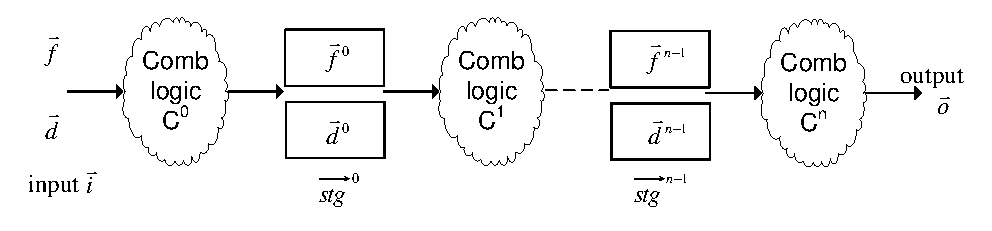
\includegraphics[width=\textwidth]{pipemod1}
\end{center}
\caption{A general structure of the encoder with pipeline stages and flow control mechanism}
  \label{fig_pipeenc}
\end{figure}


% Thus,
% each $C^j$ can be seen as a small encoder that computes $\vec{stg}^j$ or $\vec{o}$
% from $\vec{stg}^{j-1}$ or $\vec{i}$.

In the remainder of this paper,
superscript always means the pipeline stage,
while the subscript,
as mentioned in Subsection \ref{subsec_fsm},
always means the step index in the unrolled transition function.
For example,
$\vec{stg}^j$ is the $j$-th pipeline stage.
While $\vec{stg}^j_i$ is the value of this $j$-th pipeline stage 
at the $i$-th step in the unrolled state transition sequence.

\subsection{Algorithm framework}

With the encoder model shown in Figure \ref{fig_pipeenc},
our overall algorithm framework is:

\begin{enumerate}
 \item Calling Algorithm \ref{alg_fofc} to partition $\vec{i}$ into $\vec{f}$ and $\vec{d}$.
 \item Calling Algorithm \ref{algo_infer} to infer $valid(\vec{f})$ that enables $\vec{d}$ 
 to be uniquely determined with parameters $p$, $l$ and $r$.
 \item In Section \ref{sec_pipeinfer}, 
 finding out $\vec{f}^j$ and $\vec{d}^j$ in each pipeline stage $\vec{stg}^j$. 
 \item In Section \ref{sec_char}, 
 characterizing the decoder's Boolean functions that recover each pipeline stages $\vec{stg}^j$
 and input vector $\vec{i}$.
\end{enumerate}



\section{Inferring the encoder's pipeline structure}\label{sec_pipeinfer}

% \subsection{Inferring $p$, $l$ and $r$}\label{subsec_inferplr}
% Before inferring the pipeline stages,
% we first apply the algorithm of \cite{ShenTCAD11} to infer the value of $p$, $l$ and $r$ that can make the 
% output sequence $<o_{p},\dots,o_{p+l+r}>$ uniquely determine all $i_{p+l}\in \vec{i}_{p+l}$.
% This algorithm iteratively increase a parameter $b$,
% and set $p$, $l$ and $r$ all to $b$,
% until $F_{PC}(p,l,r)$ become unsatisfiable for all $i_{p+l}\in \vec{i}_{p+l}$.

\subsection{Minimizing $r$ and $l$}\label{reduceing}

\begin{algorithm}[t]
\SetAlgoVlined
\For{$r':=r \to 0$} {
\ShowLnLabel{testr_1}
  \If{$r'\equiv 0$ or $F_{PC}(p,l,r'-1)\wedge valid(\vec{f}_{p+l})$ is satisfiable for some $i\in \vec{i}$} {
    break
  }
}
return $r'$
\caption{Minimizing $r$}
\label{algo_remove2}
\end{algorithm}

As Algorithm \ref{algo_infer} increases $p$, $l$ and $r$ simultaneously,
there may be some redundancy in the value of $l$ and $r$.
So we need to first minimize $r$ in Algorithm \ref{algo_remove2}.


% To simplify the presentation,
% we will only introduce the $r$ case.
In Line \ref{testr_1},
we enforce the inferred flow control predicate $valid(\vec{f})$ by
conjugating it with $F_{PC}(p,l,r'-1)$.
When it is satisfiable,
then $r'$ is the last one that makes $F_{PC}(p,l,r')\wedge valid(\vec{f}_{p+l})$ unsatisfiable,
we return it directly.
On the other hand,
when $r'\equiv 0$,
$F_{PC}(p,l,0)$ must have been tested in last iteration,
and the result must be unsatisfiable.
In this case we return $0$.

% Minimizing $l$ is similar but with two exceptions:
% First, 
% the range of $l'$ to be enumerated contains some negative value,
% which means $i$ only depend on the value of $o$ in the future.
% Second,
% to be compatible with such cases,
% we use a new formula $F'_{PC}$ in Line \ref{testr_2}.
% When $l\ge 0$,
% $F'_{PC}$ equals to $F_{PC}$.
% But when $l<0$,
% $F'_{PC}$ is define below:
% 
% \begin{multline}\label{uniqt11}
% % \begin{split}
% F'_{PC}(p,l,r):=\\
% \left\{
% \begin{array}{cc}
% &\bigwedge_{m=0}^{p+l+r}
% \{
% (\vec{s}_{m+1},\vec{o}_m)\equiv T(\vec{s}_m,\vec{i}_m)
% \}
% \\
% \wedge&\bigwedge_{m=0}^{p+l+r}
% \{
% (\vec{s'}_{m+1},\vec{o'}_m)\equiv T(\vec{s'}_m,\vec{i'}_m)
% \}
% \\
% \wedge&\bigwedge_{m=p-l}^{p+r}\vec{o}_m\equiv \vec{o'}_m \\
% \wedge& i_{p}\equiv 1 \wedge  i'_{p}\equiv 0 
% % \wedge&\bigwedge_{m=0}^{p+l+r}assertion(\vec{i}_m) \\
% % \wedge&\bigwedge_{m=0}^{p+l+r}assertion(\vec{i'}_m) 
% \end{array}
% \right\}
% % \end{split}
% \end{multline}
% 
% The only change of Equation (\ref{uniqt11}) compared to Equation (\ref{uniqt1})
% are that 
% the range of output vector is change to $p-l\le m\le p+r$,
% while the subscripts of $i$ and $i'$ in the last line refer to $p$ only,
% $l$ are removed.

Now, 
we have a minimized $r$ from Algorithm \ref{algo_remove2},
which can make $\vec{i}_{p+l}$ to be uniquely determined by $<\vec{o}_{p},\dots,\vec{o}_{p+l+r}>$.

\begin{figure}[t]
\begin{center}
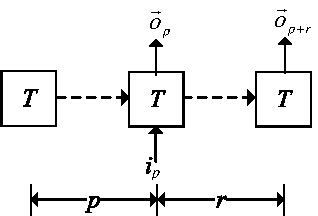
\includegraphics[width=0.5\textwidth]{pc1}
\end{center}
\caption{Recovering input with reduced output sequence}
  \label{fig_pc1}
\end{figure}

We further require that :
\begin{enumerate}
 \item As shown in Figure \ref{fig_pc1},
 $l$ can be reduced to 0,
 which means $\vec{i}_{p}$ can be uniquely determined by $<\vec{o}_{p},\dots,\vec{o}_{p+r}>$,
 that is,
 the set of future outputs.
 \item The above mentioned output sequence $<\vec{o}_{p},\dots,\vec{o}_{p+r}>$ 
 can be further reduced to $\vec{o}_{p+r}$.
 This means $\vec{o}_{p+r}$ is the only output vector needed to recover the input vector $\vec{i}_p$.
\end{enumerate}

Checking these two requirements
equals to checking the unsatisfiability of $F'_{PC}(p,r)\wedge valid(\vec{f}_{p+l})$,
with $F'_{PC}(p,r)$ defined below:

\begin{equation}\label{uniqt11}
% \begin{split}
F'_{PC}(p,r):=
\left\{
\begin{array}{cc}
&\bigwedge_{m=0}^{p+r}
\{
(\vec{s}_{m+1},\vec{o}_m)\equiv T(\vec{s}_m,\vec{i}_m)
\}
\\
\wedge&\bigwedge_{m=0}^{p+r}
\{
(\vec{s'}_{m+1},\vec{o'}_m)\equiv T(\vec{s'}_m,\vec{i'}_m)
\}
\\
\wedge&\vec{o}_{p+r}\equiv \vec{o'}_{p+r} \\
\wedge& i_{p}\equiv 1 \wedge  i'_{p}\equiv 0 
% \wedge&\bigwedge_{m=0}^{p+l+r}assertion(\vec{i}_m) \\
% \wedge&\bigwedge_{m=0}^{p+l+r}assertion(\vec{i'}_m) 
\end{array}
\right\}
% \end{split}
\end{equation}


This equation seems much stronger than the general requirement in Equation (\ref{uniqt1}).
But we will show in experimental results that 
they are always fulfilled.



\subsection{Inferring pipeline stages}\label{subsec_inferstage}

Now,
with the inferred $p$ and $r$,
we need to generalize $F'_{PC}$ in Equation (\ref{uniqt11}) to the following new formula that
can determine whether a particular variable $v$ at step $j$
can be uniquely determined by a vector $\vec{w}$ at step $k$.
Now $v$ and $\vec{w}$ can be either input, registers or output variables.

\begin{equation}\label{uniqt2}
% \begin{split}
F''_{PC}(p,r,v,j,\vec{w},k):=
\left\{
\begin{array}{cc}
&\bigwedge_{m=0}^{p+r}
\{
(\vec{s}_{m+1},\vec{o}_m)\equiv T(\vec{s}_m,\vec{i}_m)
\}
\\
\wedge&\bigwedge_{m=0}^{p+r}
\{
(\vec{s'}_{m+1},\vec{o'}_m)\equiv T(\vec{s'}_m,\vec{i'}_m)
\}
\\
\wedge&\vec{w}_{k}\equiv \vec{w'}_{k} \\
\wedge& v_{j}\equiv 1 \wedge  v'_{j}\equiv 0 
% \wedge&\bigwedge_{m=0}^{p+l+r}assertion(\vec{i}_m) \\
% \wedge&\bigwedge_{m=0}^{p+l+r}assertion(\vec{i'}_m) 
\end{array}
\right\}
% \end{split}
\end{equation}

Obviously,
when $F''_{PC}(p,r,v,j,\vec{w},k)$ is unsatisfiable,
$\vec{w}_k$ can uniquely determine $v_j$.

For $0\le j\le n-1$,
in the $j$-th pipeline stage $\vec{stg}^j$,
its flow control vector $\vec{f}^j$ is exactly the set of registers $s\in \vec{s}$ 
that can be uniquely determined at the $j-((n-1)-(p+r))$-th step by $\vec{o}$ 
at the $p+r$-th step without enforcing $valid(\vec{f}_p)$.
% With Equation (\ref{uniqt2}),
It can be formally defined as:

\begin{equation}\label{stgn_fj}
\vec{f}^{j} := 
 \left\{
 s\in \vec{s} ~| 
\begin{array}{cc}
 F''_{PC}(p,r,s,j-D,\vec{o},p+r)\\
 ~is~unsatisfiable
\end{array}
\right\}
\end{equation}

with:

\begin{equation}\label{stgn_def}
\begin{array}{ccc}
% S             & := & \vec{s}/\bigcup_{j<k\le n-2}\vec{stg}^{k}\\
D             & := & (n-1)-(p+r)\\
\end{array}
\end{equation}

While the data vector $\vec{d}^j$ in the $j$-th pipeline stage $\vec{stg}^j$
is the set of registers $s\in \vec{s}$ 
that can be uniquely determined at the same $j-((n-1)-(p+r))$-th step 
by $\vec{o}$ at the $p+r$-th step by enforcing $valid(\vec{f}_p)$.
% With Equation (\ref{uniqt2}),
It can be formally defined as:

\begin{equation}\label{stgn_dj}
\vec{d}^{j} := 
 \left\{
 s\in \vec{s} ~| 
 \begin{array}{cc}
 F''_{PC}(p,r,s,j-D,\vec{stg}^{j+1},j-D+1)\wedge valid(\vec{f}_p)\\
 ~is~unsatisfiable
 \end{array}
\right\}
\end{equation}



% Similarly,
% for $0\le j\le n-2$,
% $\vec{f}^j$ at $j-((n-2)-(p+r-1))$-th step
% can be uniquely determined at the $p+r$-th step by $\vec{o}$ without enforcing $valid(\vec{f})$.
% So we can recursively defined $\vec{f}^j$ as :
% 
% \begin{equation}\label{stgn_def}
% \begin{array}{ccc}
% S             & := & \vec{s}/\bigcup_{j<k\le n-2}\vec{stg}^{k}\\
% D             & := & (n-2)-(p+r-1)\\
% \end{array}
% \end{equation}
% 
% \begin{equation}\label{stgn_j}
% \vec{stg}^{j} := 
%  \left\{
%  s\in S ~| 
% % \begin{array}{cc}
%  F''_{PC}(p,r,s,j-D,\vec{stg}^{j+1},j-D+1)
%  ~is~unsatisfiable
% % \end{array}
% \right\}
% \end{equation}
% 
% With Equation (\ref{stgn_1}) and (\ref{stgn_j}),
% all the pipeline stages can now be inferred.

% \subsection{Inferring the pipeline stage that uniquely determines input vector}\label{subsec_inferinput}
% 
% According to Figure \ref{fig_pipeenc},
% $\vec{stg}^0$ defined in Equation (\ref{stgn_j}) is
% exactly the pipeline stage that uniquely determined the input vector $\vec{i}$.
% 
% But in real encoders,
% this may not be the case.
% So we need to search for the smallest $j$ from $0$ to $n-1$ that can make $\vec{i}$ to be uniquely determined by $\vec{stg}^j$,
% that is,
% the smallest $j$ that can make $F''_{PC}(p,r,i,p,\vec{stg}^{j},j-D)$ unsatisfiable for all $i\in \vec{i}$,
% with $D$ defined in Equation (\ref{stgn_def}).

% \subsection{Finding out the flow control vectors in each pipeline stage}

\section{Characterizing the Boolean function of input variables and pipeline registers}\label{sec_char}
\subsection{Characterizing the Boolean function of the last pipeline stage}

According to Equation (\ref{stgn_fj}),
every registers $s\in \vec{f}^{n-1}$ can be uniquely determined by $\vec{o}$ at the $p+r$-th step,
that is,
$F''_{PC}(p,r,s,p+r,\vec{o},p+r)$ is unsatisfiable and can be partitioned into :

\begin{equation}
 \phi_A := 
 \left\{
\begin{array}{cc}
&\bigwedge_{m=0}^{p+r}
\{
(\vec{s}_{m+1},\vec{o}_m)\equiv T(\vec{s}_m,\vec{i}_m)
\}
\\
\wedge& s_{p+r}\equiv 1 
\end{array}
\right\}
\end{equation}

\begin{equation}
% \begin{split}
\phi_B := 
\left\{
\begin{array}{cc}
&\bigwedge_{m=0}^{p+r}
\{
(\vec{s'}_{m+1},\vec{o'}_m)\equiv T(\vec{s'}_m,\vec{i'}_m)
\}
\\
\wedge&\vec{o}_{p+r}\equiv \vec{o'}_{p+r} \\
\wedge& s'_{p+r}\equiv 0 
% \wedge&\bigwedge_{m=0}^{p+l+r}assertion(\vec{i}_m) \\
% \wedge&\bigwedge_{m=0}^{p+l+r}assertion(\vec{i'}_m) 
\end{array}
\right\}
% \end{split}
\end{equation}

As $F''_{PC}(p,r,s,p+r,\vec{o},p+r)$ equals to $\phi_A \wedge \phi_B$,
so $\phi_A \wedge \phi_B$ is unsatisfiable.
And the common variables of $\phi_A$ and $\phi_B$ is $\vec{o}_{p+r}$.

According to \cite{InterpBoolFunction},
a Craig interpolant $\phi_I$ of $\phi_A$ with respect to $\phi_B$ can be constructed,
which refer only to $\vec{o}_{p+r}$,
and covers all the valuations of $\vec{o}_{p+r}$ that can make $s_{p+r}\equiv 1$.
At the same time,
$\phi_I\wedge \phi_B$ is unsatisfiable,
which means $\phi_I$ covers nothing that can make $s_{p+r}\equiv 0$.

Thus,
$\phi_I$ can be used as the decoder's Boolean function that recovers $s\in \vec{stg}^{n-1}$ from $\vec{o}$.

By replacing $F''_{PC}(p,r,s,p+r,\vec{o},p+r)$ with $F''_{PC}(p,r,s,p+r,\vec{o},p+r)\wedge valid(f_p)$,
we can similarly characterize the Boolean function that recovers $\vec{d}^{n-1}$.

\subsection{Characterizing the Boolean function of other pipeline stages}
According to Figure \ref{fig_pipeenc},
% Similar to last subsection,
$\vec{f}^j$ at the $j-D$-step can be uniquely determined by $\vec{stg}^{j+1}$ at the $j-D+1$-th step.
So we can partition the unsatisfiable formula $F''_{PC}(p,r,s,j-D,\vec{stg}^{j+1},j-D+1)$ 
 into the following two equations:

\begin{equation}
 \phi_A := 
 \left\{
\begin{array}{cc}
&\bigwedge_{m=0}^{p+r}
\{
(\vec{s}_{m+1},\vec{o}_m)\equiv T(\vec{s}_m,\vec{i}_m)
\}
\\
\wedge& s_{j-D}\equiv 1 
\end{array}
\right\}
\end{equation}

\begin{equation}
% \begin{split}
\phi_B := 
\left\{
\begin{array}{cc}
&\bigwedge_{m=0}^{p+r}
\{
(\vec{s'}_{m+1},\vec{o'}_m)\equiv T(\vec{s'}_m,\vec{i'}_m)
\}
\\
\wedge&\vec{stg}^{j+1}_{j-D+1}\equiv \vec{stg'}^{j+1}_{j-D+1} \\
\wedge& s'_{j-D}\equiv 0 
% \wedge&\bigwedge_{m=0}^{p+l+r}assertion(\vec{i}_m) \\
% \wedge&\bigwedge_{m=0}^{p+l+r}assertion(\vec{i'}_m) 
\end{array}
\right\}
% \end{split}
\end{equation}

Again,
a Craig interpolant $\phi_I$ of $\phi_A$ with respect to $\phi_B$ can be constructed,
and used as the decoder's Boolean function that recovers $\vec{f}^{j}$ from $\vec{stg}^{j+1}$.

Similarly,
by replacing $F''_{PC}(p,r,s,j-D,\vec{stg}^{j+1},j-D+1)$  with 
$F''_{PC}(p,r,s,j-D,\vec{stg}^{j+1},j-D+1)\wedge valid(f_p)$ ,
we can characterize the Boolean function that recovers $\vec{d}^{j}$ from $\vec{stg}^{j+1}$.

\subsection{Characterizing the Boolean function of the encoder's input variables}

According to Figure \ref{fig_pipeenc},
$\vec{f}$ at the $p$-step can be uniquely determined by $\vec{stg}^0$ at the $p$-th step.
$F''_{PC}(p,r,i,p,\vec{stg}^0,p)$ is unsatisfiable and can be partitioned into :

\begin{equation}
% \begin{split}
\phi_A:=
\left\{
\begin{array}{cc}
&\bigwedge_{m=0}^{p+r}
\{
(\vec{s}_{m+1},\vec{o}_m)\equiv T(\vec{s}_m,\vec{i}_m)
\}
\\
\wedge& i_{p}\equiv 1 
% \wedge&\bigwedge_{m=0}^{p+l+r}assertion(\vec{i}_m) \\
% \wedge&\bigwedge_{m=0}^{p+l+r}assertion(\vec{i'}_m) 
\end{array}
\right\}
% \end{split}
\end{equation}

\begin{equation}
% \begin{split}
\phi_B:=
\left\{
\begin{array}{cc}
&\bigwedge_{m=0}^{p+r}
\{
(\vec{s'}_{m+1},\vec{o'}_m)\equiv T(\vec{s'}_m,\vec{i'}_m)
\}
\\
\wedge&\vec{stg}^0_p\equiv \vec{stg'}^0_p \\
\wedge& i'_{p}\equiv 0 
% \wedge&\bigwedge_{m=0}^{p+l+r}assertion(\vec{i}_m) \\
% \wedge&\bigwedge_{m=0}^{p+l+r}assertion(\vec{i'}_m) 
\end{array}
\right\}
% \end{split}
\end{equation}

Again,
the Craig interpolant $\phi_I$ of $\phi_A$ with respect to $\phi_B$ 
can be used as the decoder's Boolean function that recovers $\vec{f}$ from $\vec{stg}^0$.

Similarly,
by replacing $F''_{PC}(p,r,i,p,\vec{stg}^0,p)$ with $F''_{PC}(p,r,i,p,\vec{stg}^0,p)\wedge valid(\vec{f}_p)$,
we can characterize the Boolean function that recovers $\vec{d}$ from $\vec{stg}^0$.



\section{Experimental results}\label{sec_exp}
We have implemented these algorithms in OCaml language,
and solved the generated CNF formulas with MiniSat 1.14 \cite{EXTSAT}.
All experiments have been run on a server with 16 Intel Xeon E5648 processors at 2.67GHz, 
192GB memory, and CentOS 5.4 Linux.
% All these experimental results and programs can be downloaded 
% from https://github.com/shengyushen/compsyn.

% \subsection{Benchmarks}
%  shows all benchmarks used in this paper.
% They come from \cite{ShenTCAD12}.
%  \item The benchmark package sent to us by Liu, the author of \cite{LiuTCAD12}.
%  So there may be some overlap between (2) and (3).
% \end{enumerate}

Table \ref{tab_bench} shows the benchmarks used in this paper.
% They are listed in the order of circuit area.
The 2nd and 3rd column show respectively the number of inputs, outputs and registers of each benchmark.
The 4th column shows the area of the encoder when mapped to LSI10K library with Design Compiler.
% We use Design compiler here instead of ABC \cite{ABC} used by other researchers 
% because ABC can not read in verilog files with registers generated by our algorithms.
In this paper, 
all area and delay are obtained in the same setting.
% we can compare them to that of \cite{LiuTCAD12}.



\begin{table*}[t]
\caption{Benchmarks and experimental results}
\begin{tabular}{|c|c|c|c|c|c|c|c|c|c|c|c|}
\hline
 Names     & \multicolumn{4}{|c|}{The encoders}                                  &   \multicolumn{3}{|c|}{decoder gener-}             &   \multicolumn{4}{|c|}{decoder gener-} \\    
           & \multicolumn{4}{|c|}{}                                              &   \multicolumn{3}{|c|}{ated by \cite{ShenTCAD11}}  &   \multicolumn{4}{|c|}{ated by this paper} \\\cline{2-12}
           &    \#   &   \#    &area  & Description                             &run  &delay&area                                    &run  &delay&area&\#\\
           & in/out  &  reg    &      &   of Encoders                            &time &(ns) &                                        &time &(ns) &    &reg\\\hline\hline
 pcie      & 10/11   & 23      & 326  &PCIE 2.0 \cite{pcie21}                    &0.37 &7.20 &624                                     &3.57 & 5.89&652 &9/12\\\hline
 xgxs      & 10/10   & 16      & 453  &     Ethernet clause 48 \cite{IEEE8023_S4}&0.21 &7.02 &540                                     &1.57 & 5.93&829 &13\\\hline
 t2eth     & 14/14   & 49      & 2252 &    Ethernet clause 36 \cite{IEEE8023_S4} &12.7 &6.54 &434                                     &47.2 & 6.12&877 &8/8/10/20\\\hline
scram.     &64/64    & 58      & 1034 & inserting 01 flipping                    &     \multicolumn{7}{|c|}{no pipeline }\\\cline{1-5}
 xfi       & 72/66   & 72      & 7772 &     Ethernet clause 49 \cite{IEEE8023_S4}&     \multicolumn{7}{|c|}{stages found}\\\hline
\end{tabular}\label{tab_bench}
\end{table*}


% \begin{table}[t]
% \caption{Experimental results}
% \begin{tabular}{|c|c|c|c|c|c|c|c|}
% \hline
%            
%  Na-       
%  mes       
%            
%  pcie      &0.37 &7.20 &624 &3.57 & 5.89&652 &9/12\\\hline
%  xgxs      &0.21 &7.02 &540 &1.57 & 5.93&829 &13\\\hline
%  t2eth     &12.7 &6.54 &434 &47.2 & 6.12&877 &8/8/10/20\\\hline
%  scr.      &     \multicolumn{7}{|c|}{no pipeline }\\\cline{1-1}
%  xfi       &     \multicolumn{7}{|c|}{structure found}\\\hline
% \end{tabular}\label{tab_res}
% \end{table}


% Table \ref{tab_res} compares the old algorithm from \cite{ShenTCAD11} to this paper's algorithm.
The 6th to 8th columns show respectively the run time of \cite{ShenTCAD11}'s algorithm to generate the decoder without pipeline,
and the delay and area of the generated decoder.
While the 9th to 11th columns show respectively the run time of this paper's algorithm to generate the pipelined decoder,
and the delay and area of the generated decoder.
The last column shows the number of registers in each pipeline stage.

Comparing the 7th and the 10th column indicates that
the decoders' delay have been significantly improved.
And the the last column shows that there actually exist very deep pipeline,
especially the t2eth with 4 pipeline stages.

One thing that is a little bit surprise is,
the two largest benchmarks scrambler and xfi do not have pipeline stages inside.
We study their code and confirm that this is true.
Their area are so large because they use much wider datapaths with 64 to 72 bits.
% Please refer to IEEE 802.3ae clause 49 \cite{IEEE8023_S4}  for more details.

\section{RELATED PUBLICATIONS}\label{sec_relwork}
%\subsection{Complementary Synthesis}
%%Complementary synthesis is an emerging new research topic,
%%there are only two papers that discuss this problem.
%
%The concept of complementary synthesis was first proposed by us\cite{ShengYuShen:iccad09} in ICCAD 2009.
%Its major shortcomings are that it is incomplete,
%and its run-time overhead of building decoder is too large.
%
%The incomplete problem has been addressed by \cite{ShengYuShen:fmcad10}, while \cite{ShengYuShen:tcad} addresses the second shortcoming by simplifying the SAT instance with unsatisfiable core extraction before building decoders.

\subsection{Complementary synthesis}\label{subsec_compsyn_relat}
The first complementary synthesis algorithm was proposed by \cite{ShenICCAD09}.
It checks the decoder's existence by iteratively increasing the bound of unrolled transition function sequence,
and generates the decoder's Boolean function by enumerating all satisfying assignments of the decoder's output.
Its major shortcomings are that it may not halt and that it has large runtime overhead
in building the decoder.

Shen et al.\cite{ShenTCAD11} and Liu et al.\cite{LiuICCAD11} tackled the halting problem independently by searching for loops in the state sequence,
while the runtime overhead problem was addressed in \cite{ShenTCAD12,LiuICCAD11} by Craig interpolant\cite{interp_McMillan}.

Shen et al.\cite{ShenTCAD12} automatically inferred an assertion for configuration pins, 
which can lead to the decoder's existence.
% It can be seen as a special case of Algorithm \ref{algo_pcln} in Section \ref{sec_infer},
% with the restriction that the inferred assertion must hold on all cycles,
% to prevent the encoder from leaving the unique state set.

Qin et al. \cite{QinTODAES15}
proposed the first algorithm can handle encoder with flow control mechanism.

Tu and Jiang \cite{TuDAC13} proposed a break-through algorithm 
based on property directed reachability analysis\cite{BradleyVMCAI11,EenFMCAD11} 
that can take the encoder's initial state into consideration,
so that the infinite history of the encoder and the decoder can be used to generate the decoder's output.
This algorithm can handle some special encoders that cannot be handled by the state-of-the-art algorithms.
But for the encoders with flow control mechanism used in our experiments,
our algorithm is enough, 
and therefore we have not implemented their algorithm in our framework.


\subsection{Program inversion}\label{subsec_proinv}
According to Gulwani \cite{dim_syn},
program inversion involves deriving a program $P^{-1}$
that negates the computation of a given program $P$.
So,
the definition of program inversion is very similar to complementary synthesis.

The initial work on deriving program inversion used proof-based approaches\cite{prog_inv},
which could handle only very small programs and very simple syntax structures.

Gl\"{u}ck et al. \cite{mtd_autoProginv} inverted first-order functional programs
by eliminating nondeterminism with LR-based parsing methods.
But,
the use of functional languages in that work is incompatible with our complementary synthesis.

{Srivastava et al. \cite{prog_inv_rev,program_inversion_11} assumed that an inverse program was typically related to the original program,
and so the space of possible inversions can be inferred by automatically
mining the original program for expressions, predicates, and control flow.
This algorithm inductively rules out invalid paths that cannot fulfill the requirement of inversion
to narrow down the space of candidate programs until only the valid ones remain.
So,
it can only guarantee the existence of a solution,
but not the correctness of this solution if its assumptions do not hold.

% \subsection{The completeness of bounded model checking}\label{subsec_bmc_relate}
% Bounded model checking(BMC) \cite{bmc_tacas99} is a model checking technology that considers only paths of limited length.
% So it is an incomplete algorithm.
% Many researchers have tried to find complete approaches for BMC.
% 
% One line of research\cite{bmc_tacas99,RecDiam} tried to find out a bound $b$,
% which can guarantee the correctness of a specification,
% if the specification is correct on all paths that are shorter than $b$.
% Line 8 of Algorithm \ref{algo_pcln} finds out the value of $p$,$d$ and $l$ that can prove the non-existence of the decoder,
% which is similar to \cite{bmc_tacas99,RecDiam}.
% 
% The other line of research\cite{kind_tacas99} tried to find a bound for induction,
% such that the correctness of a specification within any bound $b$ implies the correctness on bound $b+1$.
% Our algorithm proves the non-existence of the decoder by unfolding loops.
% This is similar to finding induction patterns \cite{kind_tacas99}.

% \textbf{This paper achieves completeness without following these two approaches.
% Instead,
% it defines two complement uniqueness conditions,
% $LP$ and $LL$,
% and find out proper algorithms to check them.}

%\subsection{Temporal Logic Synthesis}
%%Automatically synthesis of program from logic specification is first identified as Church's problem in 1962\cite{LOGARTHAUTO}.
%%Some early researches \cite{SLVSQFSS,AUTOINF} solve this problem by reducing it to checking emptiness of tree automata.
%
%The temporal logic synthesis was first addressed by Clarke et al.\cite{DSGSYNTMPLG} and Manna et al. \cite{SYNTMPLGSPC}.
%But Pnueli et al. \cite{SYNRCTVMD} pointed out that the complexity of LTL synthesis is double exponent.
%%This high complexity drives researchers turning their focus to find smaller but still useful subset of temporal logic,
%%such that synthesis problem can be solved with lower complexity.
%
%One line of research \cite{CNTLSYNTMDAUTO,DTMGENGMELTL,SYNRCTVDES} focuses on the so-called generalized reactive formulas of the form:
%$(\square \lozenge p_1 \wedge \cdots \square \lozenge p_m) \to (\square \lozenge q_1 \wedge \cdots \square \lozenge q_n)$.
%Complexity of solving synthesis problem for such formula is $O(N^3)$.
%
%The other line of research focuses on finding efficient algorithm \cite{SYNCNTLBNDRPN}
%for expensive safra determination algorithm \cite{CMPLXAUTO} on an useful formula subset,
%or just avoiding it\cite{NEWALGSTRGSYN}.
%
%%Yet another approach is antichain\cite{ANTICHAIN},
%%which reduces the expensive state set computation to computation on maximal and minimal elements of lattice.
%
%Based on these research works,
%some tools\cite{ANZU} that can handle small temporal formulas have been developed.
%
%All these works assume a hostile environment,
%which seems too restrictive for many applications.
%So Fisman et al. \cite{rationalsyn_tacas10}, Chatterjee et al. \cite{assguasyn_tacas07} and Ummels et al. \cite{ralgame_istta06} proposed rational synthesis algorithm,
%which assumes that each agents act to achieve their own goals instead of failing each other.


\subsection{Protocol converter synthesis}
Protocol converter synthesis is a process that automatically generates a translator between two different communication protocols.
This is relevant to our work,
because both focus on synthesizing communication circuits.

Avnit et al. \cite{converter_date08,converter_todeas09} first defined a general model for describing different protocols,
and then provided an algorithm to decide
whether there is some functionality of a protocol that cannot be translated into another.
Finally,
they synthesized a translator by computing the greatest fixed point for the update function of the buffer's control states.
Latter, 
they \cite{converter_date09} improved their algorithm with a more efficient design space exploration algorithm.


\section{Conclusions}\label{sec_conclude}
The CompSyn tool can infer correct assertions and generate decoder circuits for several complex encoders.
Furthermore,
it can significantly reduce the human effort in specifying assertion and selecting the correct decoder.


% \section*{Acknowledgment}
% The authors would like to thank the anonymous reviewers for their hard work.

% This work was funded by Projects 60603088 and 61070132 supported by National Natural Science Foundation of China.


\bibliographystyle{abbrv}
\bibliography{ssy}


% \begin{thebibliography}{4}
% 
% \end{thebibliography}



\end{document}
